\usetikzlibrary{shapes}

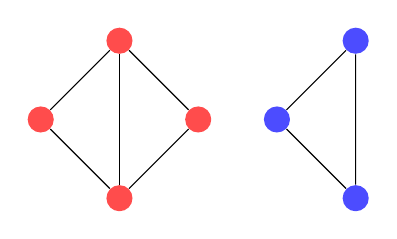
\begin{tikzpicture}[scale=1, transform shape]

  % Primer conjunto (rojo)
  \begin{scope}[every node/.style={circle, fill=red!70}]
    \node (a) at (0,0) {};
    \node (b) at (1,1) {};
    \node (c) at (2,0) {};
    \node (d) at (1,-1) {};
  \end{scope}

  \draw (a) -- (b) -- (c) -- (d) -- (a);
  \draw (b) -- (d);

  % Segundo conjunto (azul)
  \begin{scope}[xshift=3cm, every node/.style={circle, fill=blue!70}]
    \node (e) at (0,0) {};
    \node (f) at (1,1) {};
    \node (g) at (1,-1) {};
  \end{scope}

  \draw (e) -- (f) -- (g) -- (e);

\end{tikzpicture}
